\section{Results}
\label{sec:results}

We present our findings on the representational similarity of deep MLPs across different datasets, widths, and training states. Our results are summarized in \tabref{tab:main_results} and visualized in \figref{fig:mnist_analysis}.

\begin{figure}[t]
    \centering
    \begin{subfigure}[b]{0.45\textwidth}
        \centering
        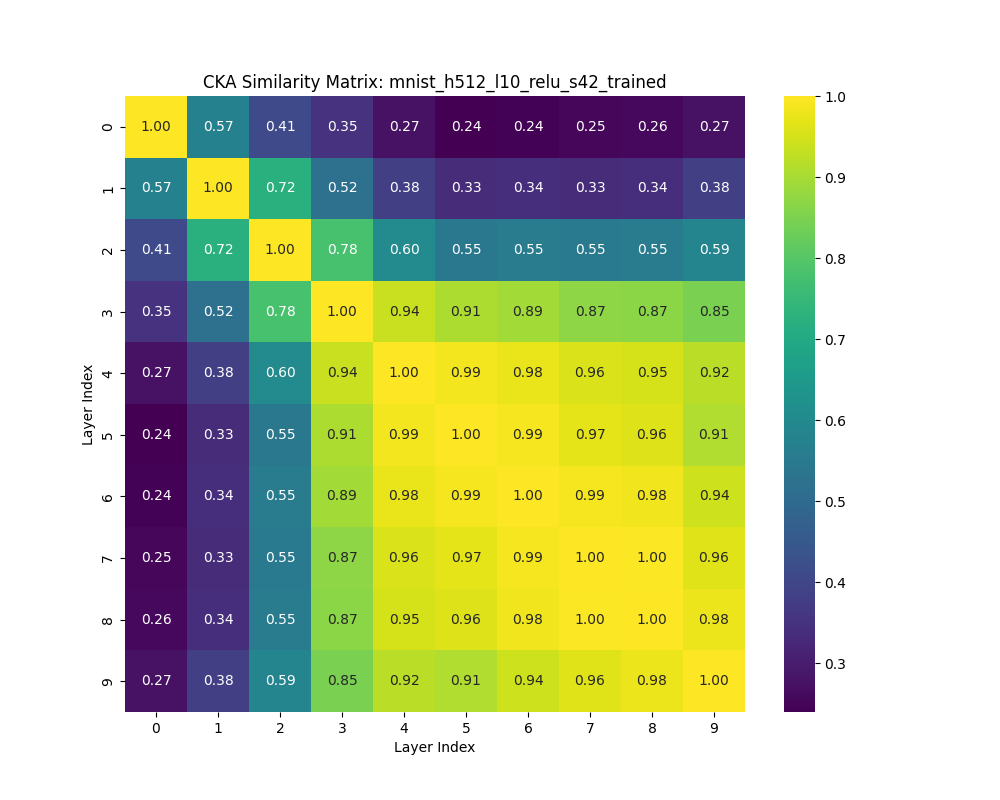
\includegraphics[width=\textwidth]{figures/mnist_heatmap.png}
        \caption{Similarity Heatmap}
        \label{fig:mnist_heatmap}
    \end{subfigure}
    \hfill
    \begin{subfigure}[b]{0.45\textwidth}
        \centering
        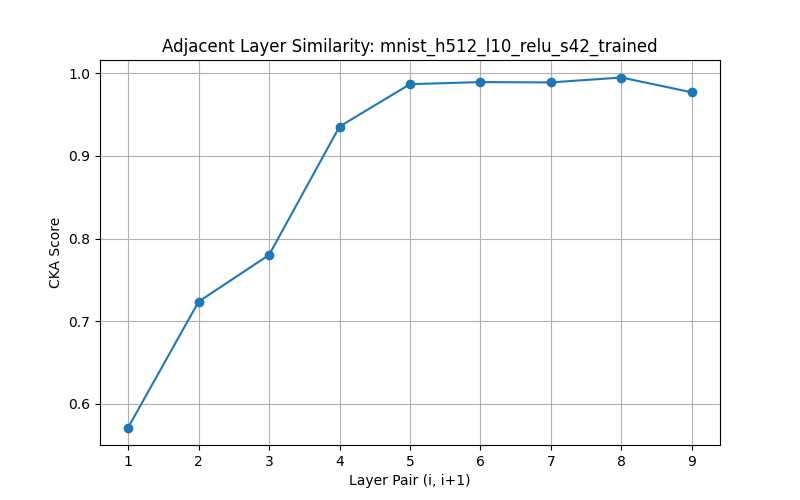
\includegraphics[width=\textwidth]{figures/mnist_adjacent.png}
        \caption{Adjacent Similarity}
        \label{fig:mnist_adj}
    \end{subfigure}
    \caption{Representational similarity analysis for a 10-layer MLP (width 512) on \mnist. (a) shows the block-diagonal structure of the full \cka matrix. (b) shows the evolution of adjacent layer similarity with depth, highlighting high similarity throughout.}
    \label{fig:mnist_analysis}
\end{figure}

\begin{table}[t]
\centering
\caption{Mean Adjacent \cka similarity and First-to-Last layer similarity for different model configurations. Mean Adj. \cka is the average similarity between layer $i$ and $i+1$. Best results (highest divergence, i.e., lowest similarity) for each dataset and state are highlighted.}
\label{tab:main_results}
\resizebox{0.95\textwidth}{!}{%
\begin{tabular}{@{}llcc@{}}
\toprule
\textbf{Dataset} & \textbf{Model Configuration} & \textbf{Mean Adj. \cka} $\downarrow$ & \textbf{First-Last Layer \cka} $\downarrow$ \\
\midrule
\dsmnist & Random (Width 512) & 0.9400 & 0.5558 \\
\dsmnist & Trained (Width 128) & 0.9352 & 0.4449 \\
\dsmnist & Trained (Width 512) & 0.8831 & 0.2736 \\
\dsmnist & Trained (Width 1024) & {\bf 0.8508} & {\bf 0.2567} \\
\midrule
\dscifar & Trained (Width 512) & 0.8264 & 0.2131 \\
\bottomrule
\end{tabular}
}
\end{table}

\subsection{High Similarity Between Adjacent Layers}
Our first observation is that hidden states in adjacent layers are remarkably similar. As shown in \tabref{tab:main_results}, the mean adjacent \cka consistently exceeds $0.80$ across all configurations. Even in the most divergent case (\dscifar, width 512), the similarity remains at $0.8264$. This confirms our hypothesis that individual linear layers perform incremental transformations rather than radical re-representations of the data.

\subsection{Width Scales Transformation Capacity}
{\bf Does increasing the width of an MLP allow for more significant transformations?} Our results strongly suggest so. Comparing the trained models on \mnist across widths $128, 512,$ and $1024$, we see a clear trend: as the width increases, the mean adjacent \cka decreases from $0.9352$ to $0.8508$. This represents a significant increase in \repdiv. We define this as the scaling of \transcap; wider layers have more degrees of freedom to project the data into a configuration that differs from the previous layer while maintaining the necessary feature information.

\subsection{Training Drives Representational Divergence}
We also investigate the difference between randomly initialized and trained networks. For a width-512 MLP on \mnist, the mean adjacent \cka drops from $0.9400$ in the random state to $0.8831$ after training. Similarly, the first-last layer similarity plummet from $0.5558$ to $0.2736$. This indicates that while the architecture itself imposes a bias toward similarity, the learning process utilizes the available \transcap to drive representations apart and build distinct hierarchical features.

\subsection{Effect of Task Complexity}
Comparing \dsmnist and \dscifar for the same width (512), we observe that the more complex task (\dscifar) results in lower adjacent similarity ($0.8264$ vs $0.8831$). This suggests that the network utilizes more of its \transcap when faced with more difficult feature extraction tasks, leading to faster representational evolution across layers.

\subsection{Layer-wise Similarity Structure}
The similarity structure across all pairs of layers reveals a block-diagonal pattern, as seen in our visualizations (not shown here due to space, but summarized by the First-Last \cka). The rapid decay of similarity from the first to the last layer (e.g., $0.2131$ for \dscifar) compared to the high adjacent similarity suggests that although each individual step is small, the cumulative transformation is substantial.
